\documentclass[a4paper, 11pt]{article}
\usepackage{comment} % enables the use of multi-line comments (\ifx \fi)
\usepackage{lipsum} %This package just generates Lorem Ipsum filler text.
\usepackage{fullpage} % changes the margin
\usepackage[utf8]{inputenc}
\usepackage{hyperref}
\usepackage{pdfpages}
\usepackage{stmaryrd}
\usepackage{graphicx}
\usepackage{subfig}

\hypersetup{
    colorlinks,
    citecolor=black,
    filecolor=black,
    linkcolor=black,
    urlcolor=black
}
\begin{document}
%Header-Make sure you update this information!!!!
\noindent
\large\textbf{Compte rendu - Indexation multimédia} \hfill \textbf{FAURE Adrien} \\
2015 - 2016

\tableofcontents

\section{Description}
Ce rapport présente mon projet d'indexation multimédia réalisé en master 2 Génie Informatique 2015 - 2016.

\section{Présentation}
La réalisation du projet suis fidèlement les étapes décrites dans le sujet.
Le projet se présente sous la forme d'un dossier contenant tout les scripts et sous dossiers nécessaire. La racine du projet présentes trois scripts essentiel ainsi que quelques dossiers clés :
\begin{itemize}
	\item \texttt{install.py} : Scripts d'installation. Créera les sous dossier nécessaire ainsi qu'un fichier de configuration relatif à l'environnement. Ce script compile également les sources annexes (lib-svm et le code des histogrammes de couleurs).
    \item \texttt{manage.py} : Point d'entré du programme, il permet d'exécuter un plan d'exécution défini pour une tache données (réaliser la chaîne complète des sift par exemple).
    \item \texttt{webapp.py} : Application web qui met à disposition deux routes http permettant l'évaluation d'un image.
    \item \texttt{rapport} : Ce dossier contient les sources latex du projet ainsi que les éléments issu des calcules (les meilleurs résultats obtenue et leurs paramétrages etc).
    \item \texttt{scripts} : Les scripts du projet. Les scripts représente les différentes étapes décrites dans le sujets. Génération des histogramme, trec\_eval, calcule des k-means etc).
    \item \texttt{plans} : Ce dossier contient les différents plans d'exécution utilisé pour le projet.
    \item \texttt{predict\_files} : Ce dossier contient les modèles nécessaire pour l'évaluation d'une image. Ce dossier n'est pas présent dans l'archive rendu car il représente trop de données. Cependant il est disponible sur la version git en ligne.
    \item \texttt{lib} et \texttt{dep} : Ces dossiers contiennent les logiciels/utilitaires annexes (djpeg,colorDescriptor ,lib\-svm et trec\_eval).
	\item \texttt{webapp} : Ce dossier contient les sources de l'IHM web en javascript et html.
\end{itemize}

\section{Présentation technique}

\subsection{Langage utilisé}
Pour réaliser le projet, j'ai choisis le langage de programmation Python. La première raison est que c'est un langage que je ne connaissais pas et que je souhaitais découvrir, par chance ce sujet de tp était réalisable en python. De plus comme pour le langage R, python est un lange réputé dans le data-mining et machine learning. La dernière raison qui motive l'utilisation de python est que je voulais essayer l'appelle de fonction native C dans un code python. Le script \texttt{histogram.py} met en place ce mécanisme avec le calcul des histogrammes de couleurs.

\subsection{Déroulement des opérations}
Comme je l'ai succinctement décris dans la première partie du rapport, le script \texttt{manage.py} situé à la racine du projet est le point d'entrée des calcules. Il permet, via des fichiers de paramétrage, de lancer les étapes nécessaires à l'analyse des concepts.
Le scripts \texttt{manage.py} présentes les options suivantes :
\begin{itemize}
	\item \texttt{-f} : Lancement du plan d'exécution spécifié en paramètre.
    \item \texttt{-d} : Lancement de tous les plans d'exécution situé dans le dossier spécifié en paramètre.
    \item \texttt{-i} : Permet de spécifier un plan d'initialisation à lancer avant de lancer les plans spécifier avec les options \texttt{-f} et \texttt{-d}
\end{itemize}

\texttt{Manage.py} présente donc un moyens de lancer les évaluations, depuis le téléchargement des images jusqu'à l'évaluation final avec trec\_eval. Il est utile de préciser que chaque exécution peu prendre du temps (plusieurs heurs , voir un jour complet avec beaucoup de plans). Afin de pouvoir suivre les étapes tout les scripts laisse une trace dans un fichier de log situé dans le dossier \texttt{log} créé lors de l'installation du projet. Ces fichiers sont importants car sans eux, il devient difficile voir impossible de débugger le programme.

Cette organisation représente une base solide pour l'analyse des images à travers les étapes imposé. En particulier, une fois qu'un plans d'exécution est bien définie pour une évaluation, par exemple pour l'évaluation des sift, il suffit de le répliquer avec autant de paramétrages différents que souhaité. L'option \texttt{-d} de \texttt{manage.py} exécutera chacun des plans du dossier qui les contient à la suite.

Chacun des scripts de calcul est construit de façon à recevoir une liste de concepts. Ce qui, on le verra plus tard permet de paralléliser les taches, car en général il n'y à pas de conflits entre les exécutions de chaque concept.

\section{Parallélisation et optimisation}

\subsection{Localisation des images}
Le projet à été réalisé dans une optique d'optimisation et de réutilisation des temps de calculs. Par exemple afin de calculer les histogrammes de couleurs de chacune des photographie le scripts
\texttt{histogram.py} télécharge une fois pour toutes les photographies mis à disposition. Si l'algorithme d'histogrammes est appelé une seconde fois le script vérifiera la présence de chacune des photographies avant d'exécuter l'analyse des couleurs. La même démarche à été adopté avec les sift. Ceci permet de pouvoir optimiser les temps de transferts réseau pour chaque exécutions.

\subsection{Factorisation des taches}
\subsubsection{Plan d'initialisation}
L'option \texttt{-i} du script \texttt{manage.py} déclenchant l'exécution d'un plan d'initialisation avant de d'exécuter le ou les plans principaux permet ainsi de factoriser certaines taches propre à un ensemble de plans.
\subsubsection{Couleur}
Pour l'évaluation des couleurs, seulement deux histogramme de couleurs sont nécessaires pour toutes les évaluation (train et val). On peut ainsi lancer le script \texttt{manage.py} avec la commande : \\ \texttt{./manage.py -d dir\_plans\_color  -i generate\_color\_histogramme.ini }.
\\ \texttt{Manage.py} exécutera alors une seul fois le plan de génération des histogrammes de couleur pour tout les plans d'évaluations des images pour les histogrammes de couleurs.
\subsubsection{Sift}

Pour l'évaluation des sift on génère un fois pour tout les plans les histogrammes des clusters au format svm. Dans le cas des sift cette option permet de gagner encore plus de temps. En effet, mes évaluations font varier le nombres de centres des k-means. Le plan d'initialisation doit ainsi générer les cluster k-means sur plusieurs dimensions (256, 512, 1024 ainsi que 2048) ainsi que les mappings et histogrammes svm. La génération d'un cluster de k-means pour 2048 centres dure environ une heure (avec un échantillonnage des sift à 1 sur 25). De plus la génération des mappings prend un certains temps. Une demi heurs pour les mappings des clusters à 256 centres et deux heures pour les mappings des cluster à 2048 centres.
Il est quasiment impensable de devoir recalculer ces informations pour chaques variations de gamma et des poids svm.

\subsection{Parallélisation des taches}

\subsubsection{Popen}
Le langage de script Python présente un api inintéressante pour l'exécution de processus en background : Le module Popen de subprocess. Cette bibliothèque python permet de lancer et contrôler des scripts ou des commande native (bash par exemple) à partir du scripts principal. En plus de pouvoir lancer des processus en background, Popen permet de récupérer leurs sorties d'erreurs ainsi que le code de retour du scripts. Ce qui permet de gérer avec p rescision leurs exécutions et ainsi d'alimenter les fichiers de logs.

\subsubsection{Taches parallélisées}
Lors de l'exécution d'un plan, chacune des étapes est conçu pour être exécutée une fois pour chaque concept. En opposition à une implémentation mono-concept, le script de génération des modèles générera les modèle de chacun des concepts donné en paramètre avant de passer à l'évaluation avec svm-predict. Une implantation mono concept exécuterais tout la chaîne d'évaluation pour un concept avant de passer au suivant. Cette information est capitale pour comprendre les taches possiblement parallélisable relative à mon implantation. Le nombre de processus désiré est en général une options préciser au script \texttt{manage.py} (-nb-threads). Afin de ne pas figer la machine, le scripts exécutera \texttt{nb-threads} processus maximum, quand un processus est terminer un nouveau peut démarrer jusqu'à la fin du programme.
Le projet permet de paralléliser les tâches suivantes :
\begin{itemize}
	\item La génération des mappings \texttt{sift -> cluster}, le traitement d'une image est parallélisé.
	\item La génération des modèles (couleur et sift), le scripts lancera en concurrence le calcul du modèle pour un concept.
	\item La génération des fichiers de concepts pour les couleurs.
\end{itemize}

D'autre taches peuvent être parallélisé, cependant cela ne représente par un grand intérêt si l'exécution pour les 20 concepts est inférieur à 10 minutes. En effet un svm-train pour un concept sift prend une dizaine de minute, et il y en à une vingtaines calculer c'est donc un gain de temps significatif. Cependant la fusion des .out lors de la fusion tardive ne prends pas plus de quelques minutes ( voir moins d'une minute) pour les vingts concepts. Une parallélisation n'est donc pas nécessaire en rapport gains de temps d'exécution contre gains de temps en programmation.

\subsection{Gestion des risques}
La gestion des risque dans un projet comme celui ci est très important. Le premier facteur à contrôler est le temps. En effet l'exécution d'un plan d'évaluation des sift pour un paramétrage donné prend environ une heure. Il est donc important de commencer en avance le projet afin de pouvoir optimiser ses résultats et ainsi permettre l'évaluation pour beaucoup de paramétrages.

La gestions des bug est également principale. En effet, durant mon projet j'ai été confronté à deux bugs importants. Comme un plan d'évaluation représente beaucoup d'enchaînements de scripts est de calcul il n'est pas toujours évident de déceler un bug. De plus il est important d'avoir une connaissance approfondit de chacun des outils que nous utilisons. Dans mon cas lors de l'évaluation par trec\_eval je téléchargeais les fichiers \texttt{.rel} avec l'utilitaire \texttt{wget}. Cependant à la première utilisation j'ai téléchargé un fichier erroné, wget par défaut ne remplace pas les fichiers existant mais crée un fichier nouveau \texttt{nomfichier.rel.1}. Ce comportement ma coûté une semaine avec de très mauvais résultats.

Une deuxième source de bug entraînant des résultats proches de zéro est la quantités importante de fichiers. En effet, lors du téléchargement des images, le réseau s'est arrêté entraînant ainsi le téléchargement incomplet d'un fichier sift. Le fichier tronqué entraînais ainsi une erreur dans les mappings de clusters sift menant finalement un décalage de 1 pour chaque images dans les histogrammes.

\section{Résultats}
\subsection{Résultats général}
Il est important de noter que le résultat présenté pour \texttt{all} représente la valeur du gain apporté pour le paramétrage permettant de trouver le meilleur compromis pour tout les résultats. Il donc pas très intéressant dans notre cas. Une valeur plus pertinente de \texttt{all} est la moyenne des évaluations pour chaque concept avec leurs meilleurs paramétrages :
\begin{itemize}
	\item sift  : 35\%;
	\item color : 17\%;
	\item fusion : 37\%.
\end{itemize}

\begin{center}
  \makebox[\textwidth]{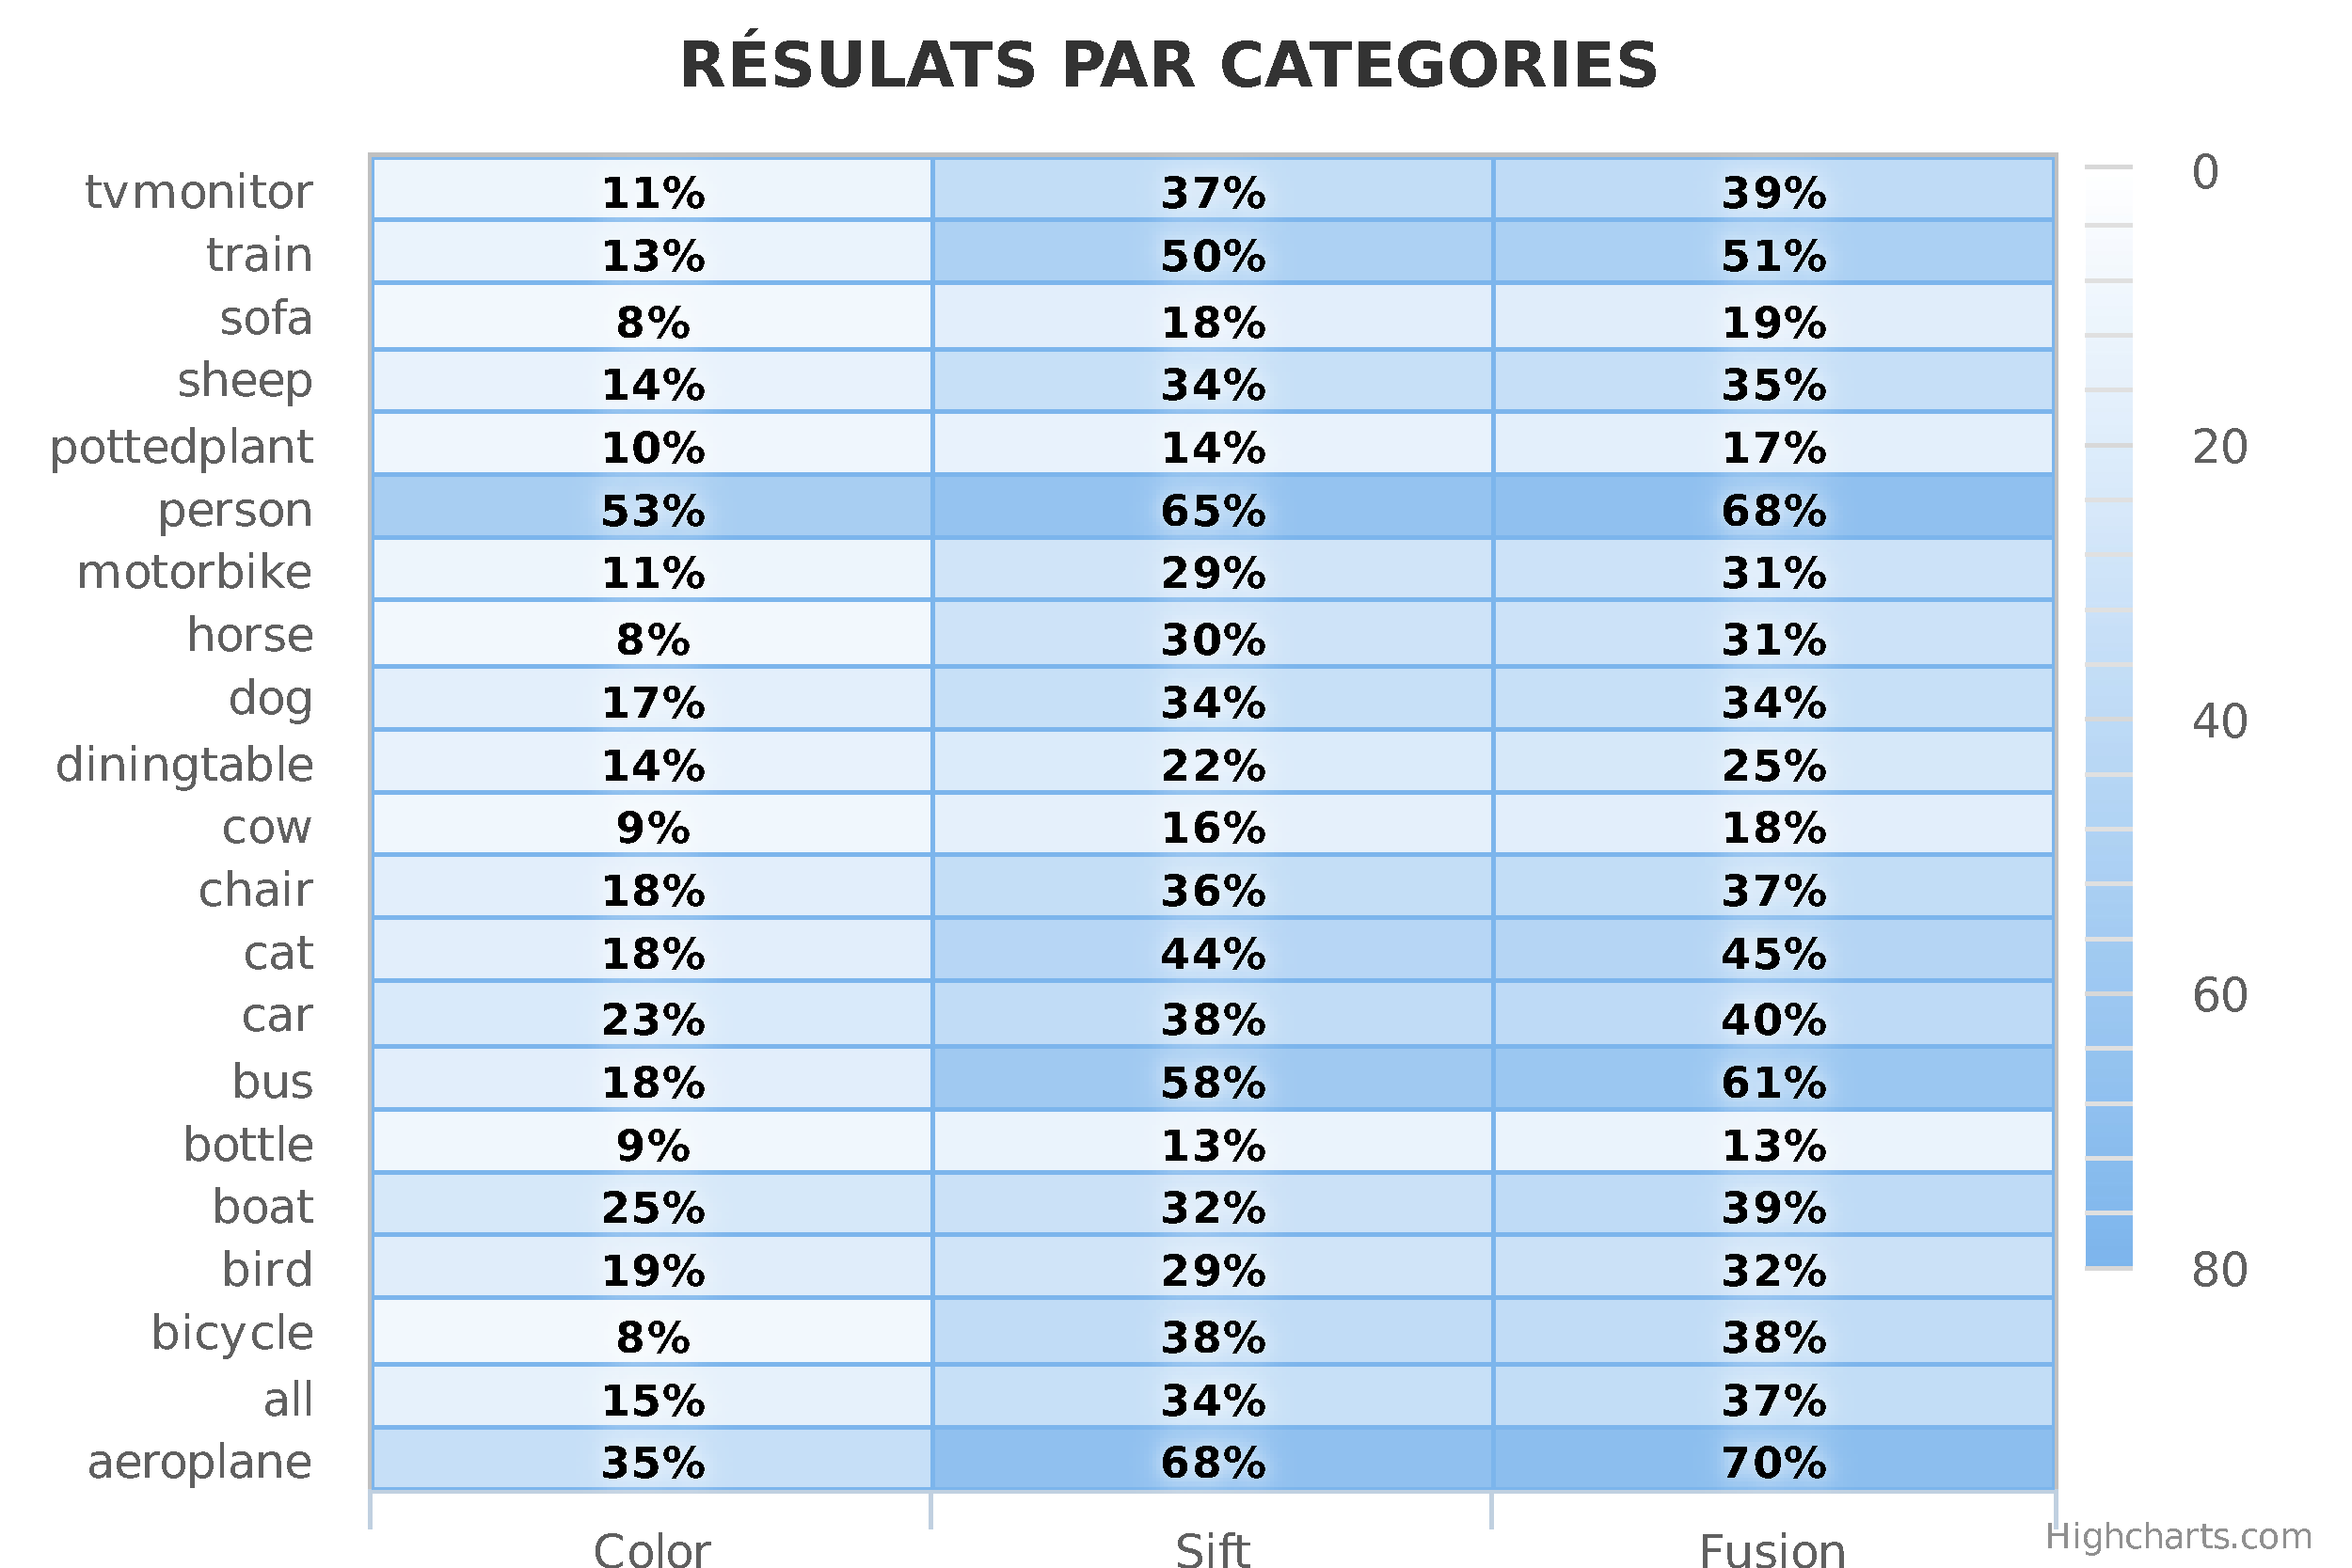
\includegraphics[scale=0.41]{chart.pdf}}
\end{center}

Voici les résultats obtenue pour chaque concept par catégorie. On observe une net amélioration au passage de couleur à sift. Avec un amélioration de 77.5\% pour \texttt{all}. Le passage de sift à fusion permet tout de même d'améliorer légèrement les résultats avec une augmentation de 8,4\%. Les évaluations par histogrammes de couleur permettent donc d'apporter une précision en plus sur le résultats général grâce à la fusion tardive.

Afin d'optimiser les résultats obtenue, les évaluations sont exécuté plusieurs fois avec des paramétrages différents.

\subsection{Résultats de l'évaluation par histogrammes de couleurs}
\begin{center}
  \makebox[\textwidth]{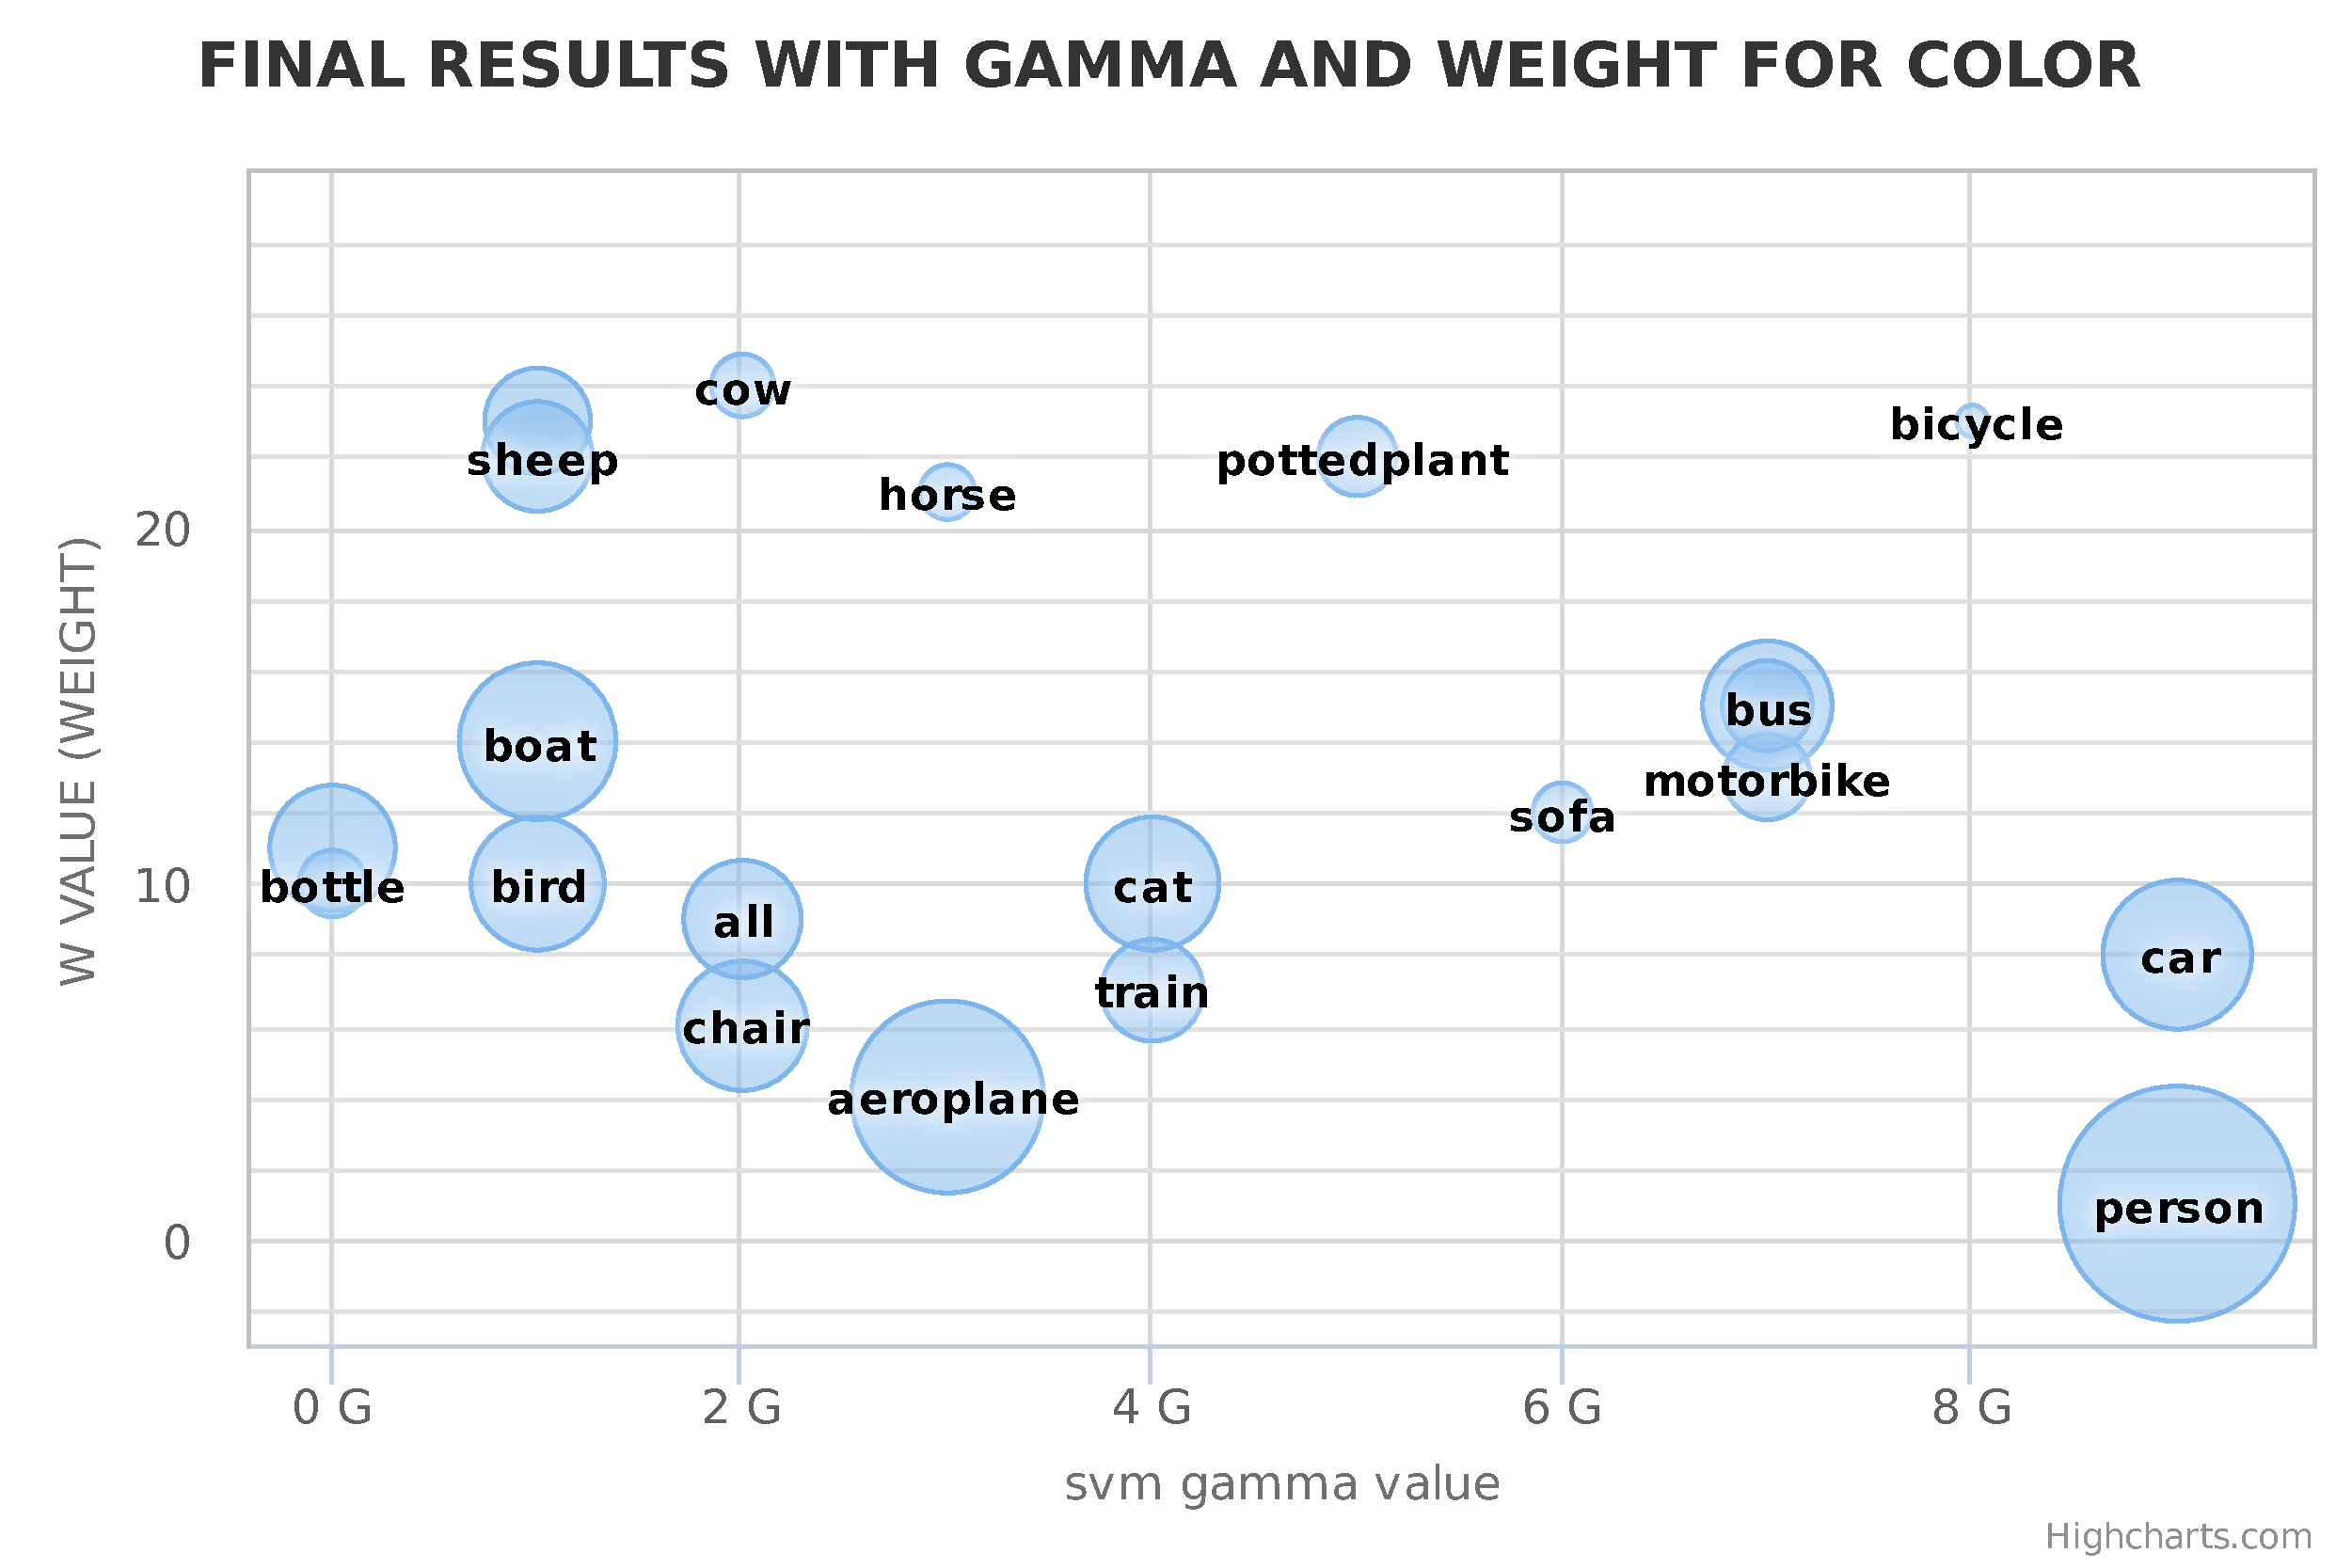
\includegraphics[scale=0.41]{color_parameters.pdf}}
\end{center}

Pour l'évaluation des couleurs, les paramètres à varier sont la valeurs gamma de svm-
train qui représente une marge d'erreur acceptable pour la séparation ainsi que le paramètre du poids attribué à un élément enregistré comme vrai dans la base d'image. Les valeurs de gamma sont choisis dans les intervalles suivants : $gamma \in \llbracket  0~;~9 \rrbracket$ et $w \in \llbracket  0~;~25 \rrbracket$.
Le diamètre du cercle représente la valeur obtenue avec l'évaluation de trec\_eval.

\subsection{Résultats de l'évaluation par sift}
Pour l'évaluation des sift, j'ai choisis de faire varier trois paramètres.
\begin{itemize}
	\item Le paramètre gamma de svm;
	\item Le poids pour un concept (paramétrage svm);
	\item Le nombre de centre du k-means.
\end{itemize}
Afin d'avoir une bonne estimation du nombre de cluster à choisir lors de la clusterisation, j'ai tracé la courbe de disparition du kmeans (valeur fournit dans l'objet kmeans du package de R).

\begin{center}
  \makebox[\textwidth]{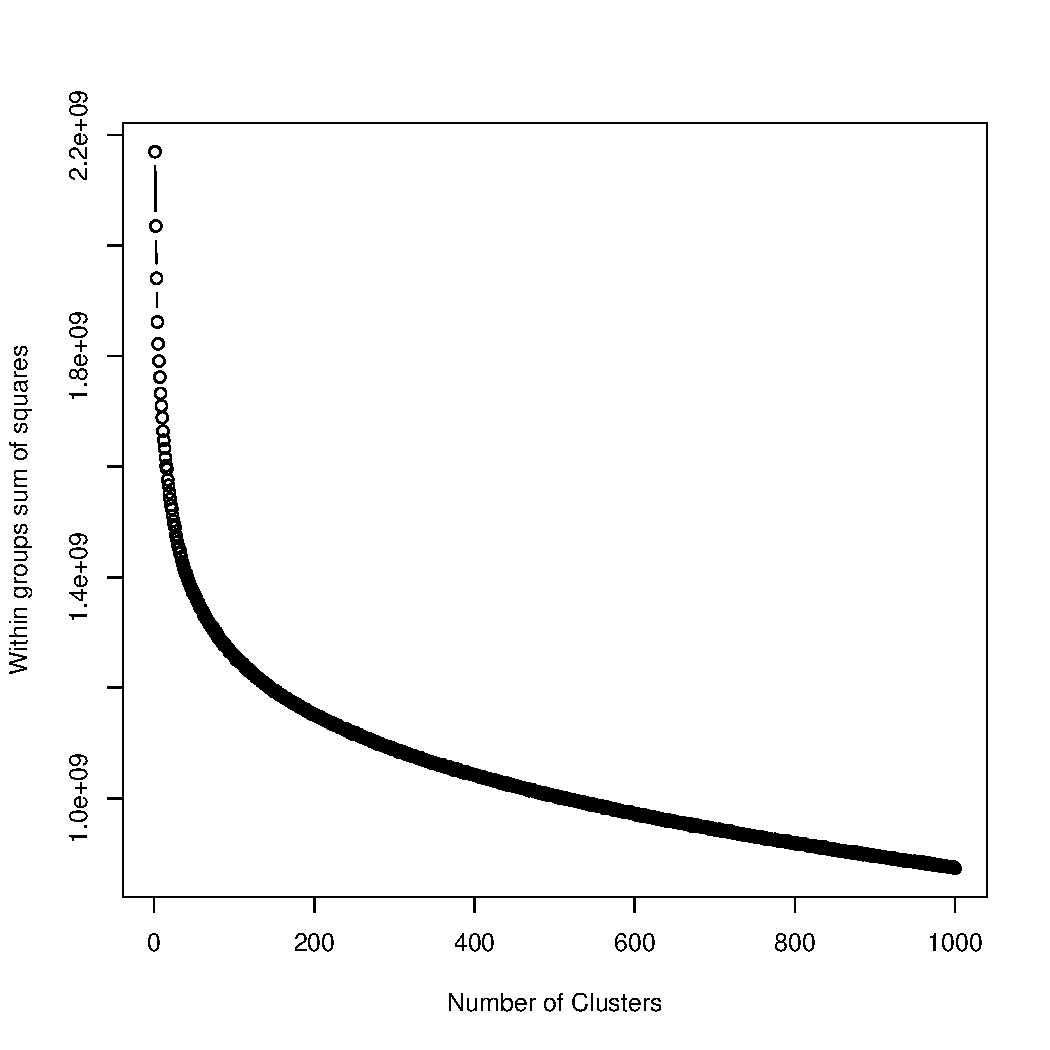
\includegraphics[scale=0.8]{Rplots.pdf}}
\end{center}

En général un "bon" nombre de cluster se situe dans la région du \texttt{coude} de cette courbe. Ainsi les clusters de 200 centres à 2000 centres représente une clusterisation de qualité. C'est pourquoi j'ai choisis de faire les évaluations pour :
$nbClusters \in \llbracket  256,512,1024,2048 \rrbracket$.


D'une façon générale, l'évaluation d'image grâce aux calculs de sift apporte de  meilleurs résultats finaux.
Les paramètres ont été selectionnés dans les ensembles :
\begin{itemize}
 \item $nbClusters \in \llbracket  256;512;1024;2048 \rrbracket$.
 \item $gamma \in \llbracket  1;25;50;150;400 \rrbracket$.
  \item $w \in \llbracket  5;20;50 \rrbracket$.
\end{itemize}

\begin{center}
\begin{tabular}{|l|c|c|c|r|}
  \hline
  concept & Nombre de centres & Gamma & w & Resultats (map) \\
  \hline
	aeroplane&1024&150 & 20 & 0.6883\\  \hline
	all&512&150 & 5 & 0.3465\\  \hline
	bicycle&512&150 & 5 & 0.3813\\  \hline
	bird&512&150 & 5 & 0.2910\\  \hline
	boat&1024&150 & 20 & 0.3273\\  \hline
	bottle&512&25 & 20 & 0.1344\\  \hline
	bus&2048&150 & 20 & 0.5828\\  \hline
	car&512&150 & 5 & 0.3818\\  \hline
	cat&512&150 & 5 & 0.4418\\  \hline
	chair&512&400 & 20 & 0.3604\\  \hline
	cow&512&150 & 5 & 0.1692\\  \hline
	diningtable&512&150 & 100 & 0.2252\\  \hline
	dog&512&150 & 5 & 0.3438\\  \hline
	horse&512&150 & 5 & 0.3091\\  \hline
	motorbike&512&400 & 20 & 0.2983\\  \hline
	person&512&400 & 20 & 0.6571\\  \hline
	pottedplant&256&100 & 20 & 0.1415\\  \hline
	sheep&2048&150 & 20 & 0.3482\\  \hline
	sofa&256&150 & 20 & 0.1834\\  \hline
	train&512&150 & 5 & 0.5052\\  \hline
	tvmonitor&2048&150 & 20 & 0.3774 \\
   \hline
\end{tabular}
\end{center}

Afin de présenter le gain de qualité j'ai dessiné le diagramme ci-dessous. Il présente pour chaque concept le gain effectif en pourcentage apporté à la prédiction des sifts.
Voici la liste des paramètres optimaux trouvé pour chaque concept :

\begin{center}
  \makebox[\textwidth]{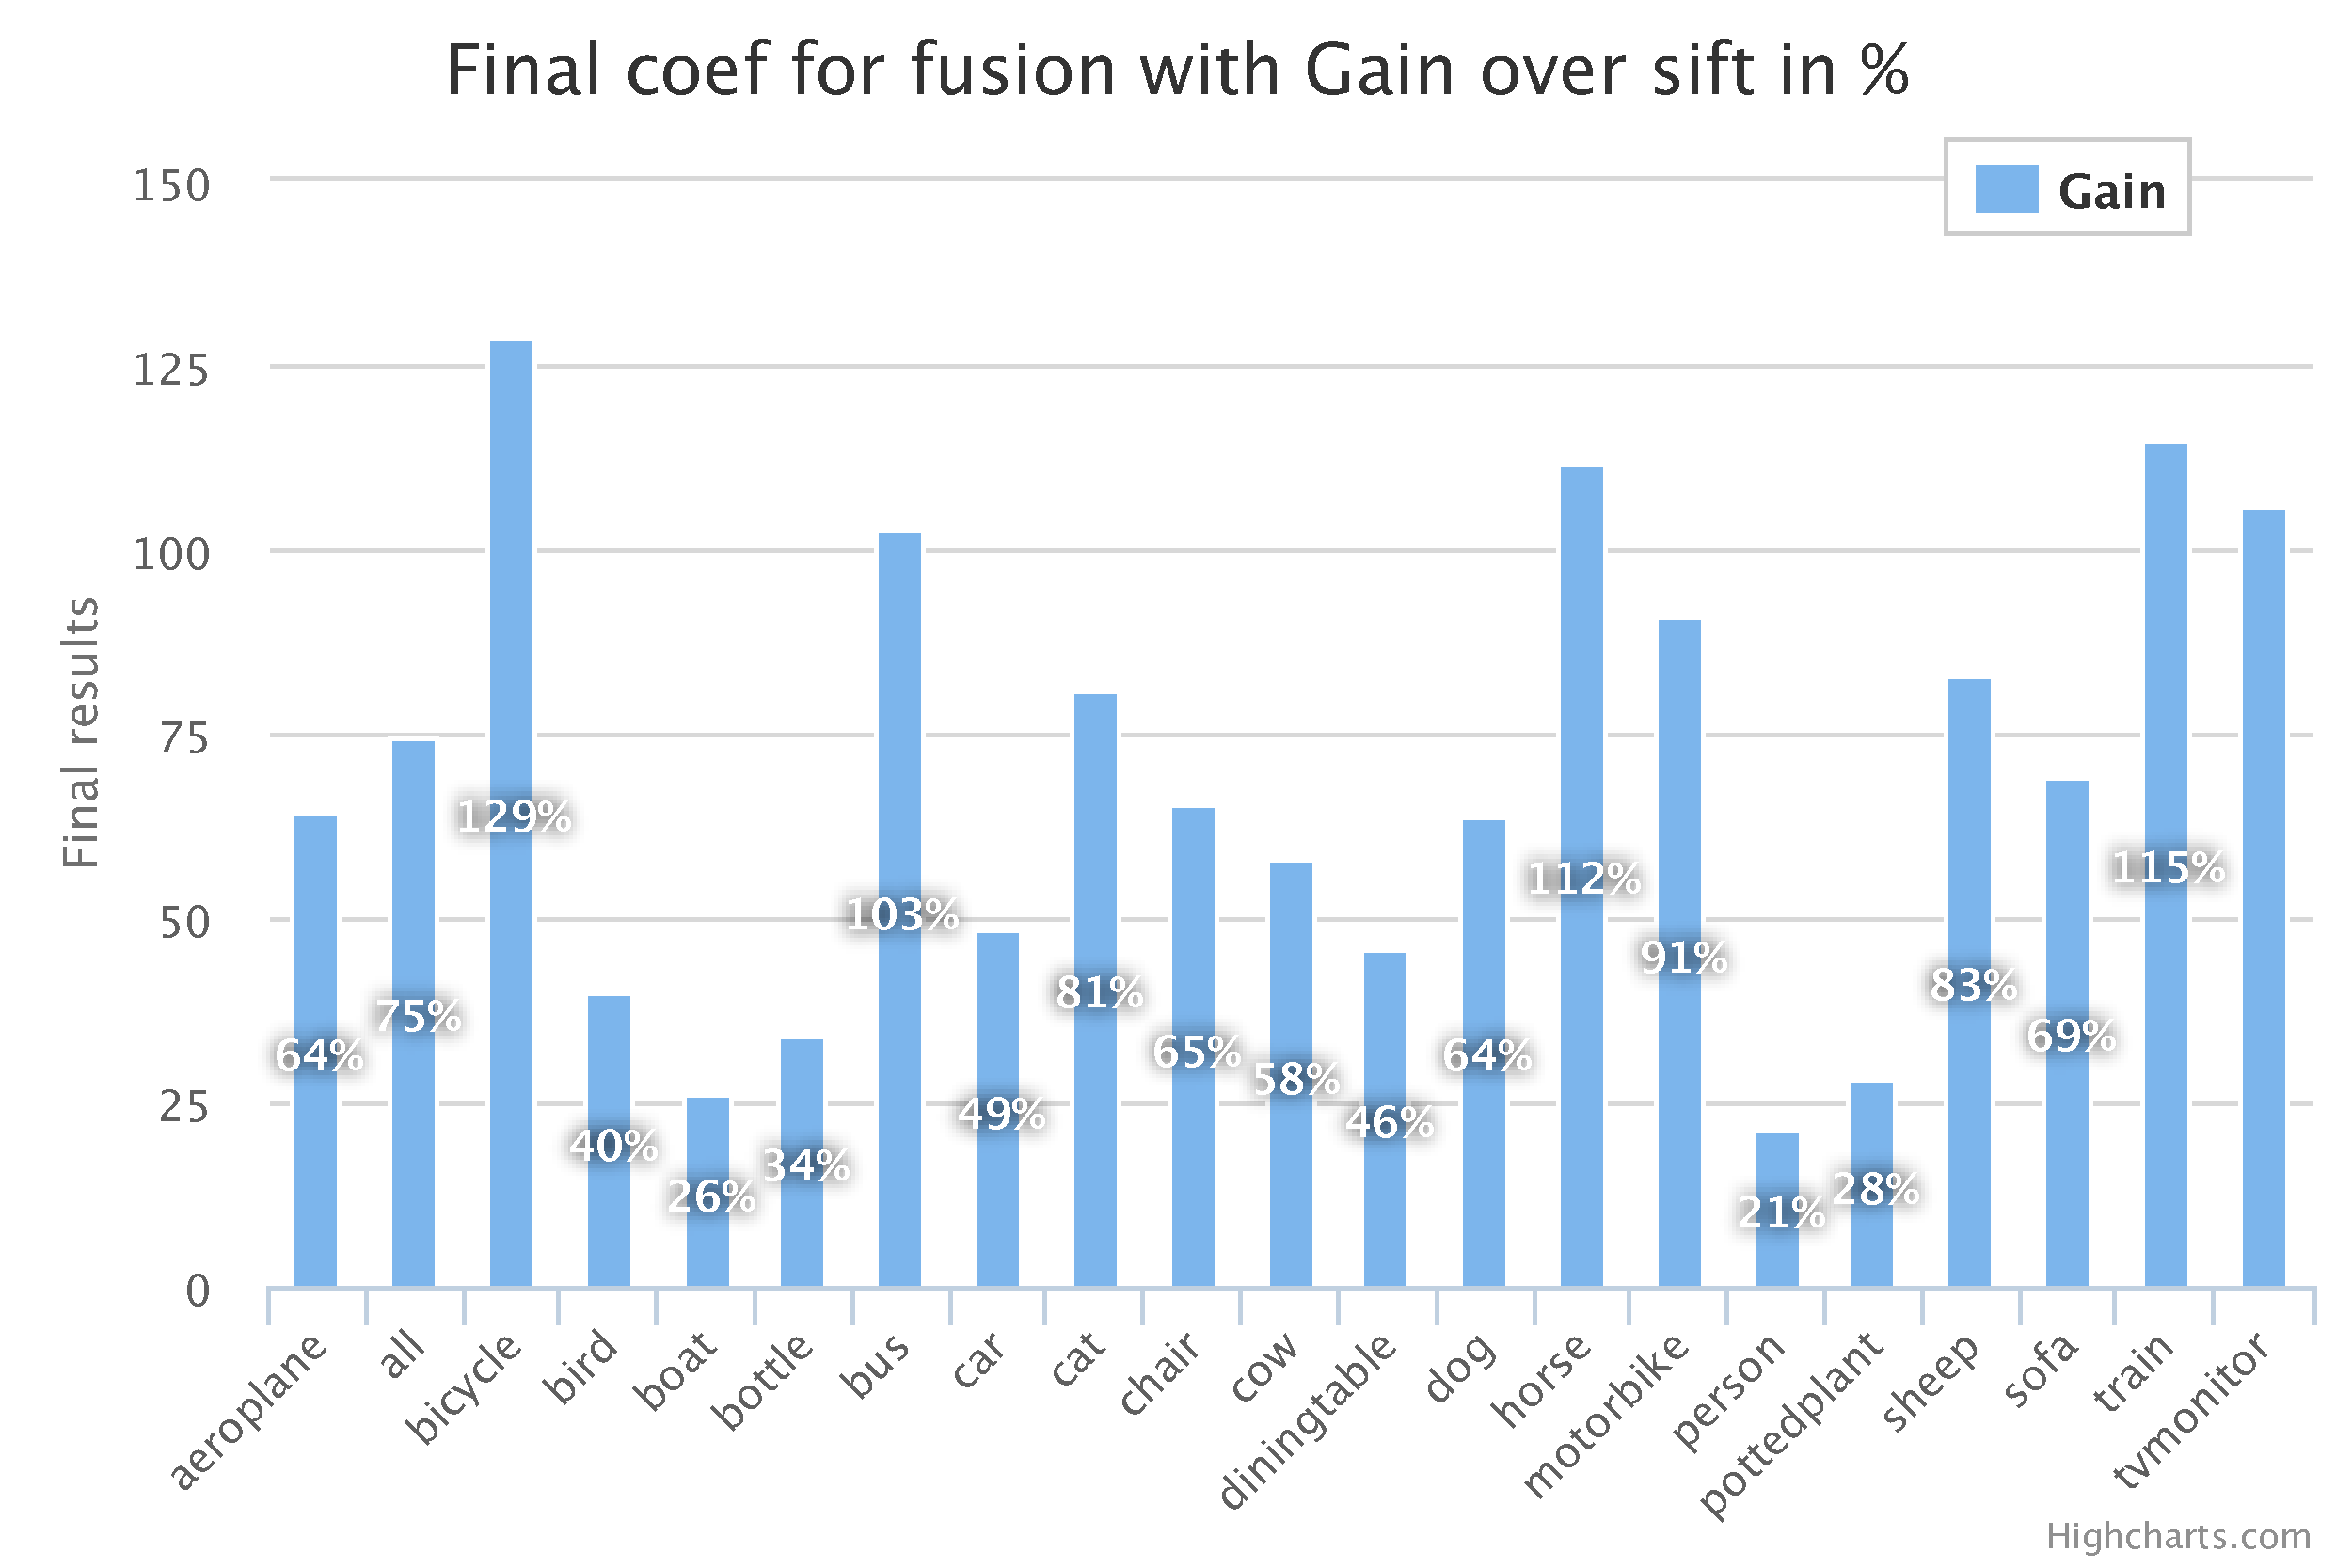
\includegraphics[scale=0.41]{sift_color_diff.pdf}}
\end{center}
Le Gain est calculé de la façon suivante :
\begin{equation}
  Gain = (| map_{sift} - map_{color} | / (map_{sift} - map_{color}) / 2) * 100
\end{equation}
La variables map est la variable correspondant au champ \texttt{map}  dans le fichier résultat de trec\_eval.

\subsection{Résultats de l'évaluation par fusion tardive}

Pour une optimisation maximal des résultats de la fusion, la fusion des fichier \texttt{.out} s'effectue depuis les fichiers issue des paramétrages ayant apporté les meilleurs résultats pour les sift et pour les couleurs.
Par exemple, pour le calcul des avions, on prendra le fichier de sortie des paramétrages ;
\begin{itemize}
	\item couleur : g = 4 et w = 3;
	\item sift : cluster de 1024 centres, g = 150 et w = 20.
\end{itemize}

\begin{center}
  \makebox[\textwidth]{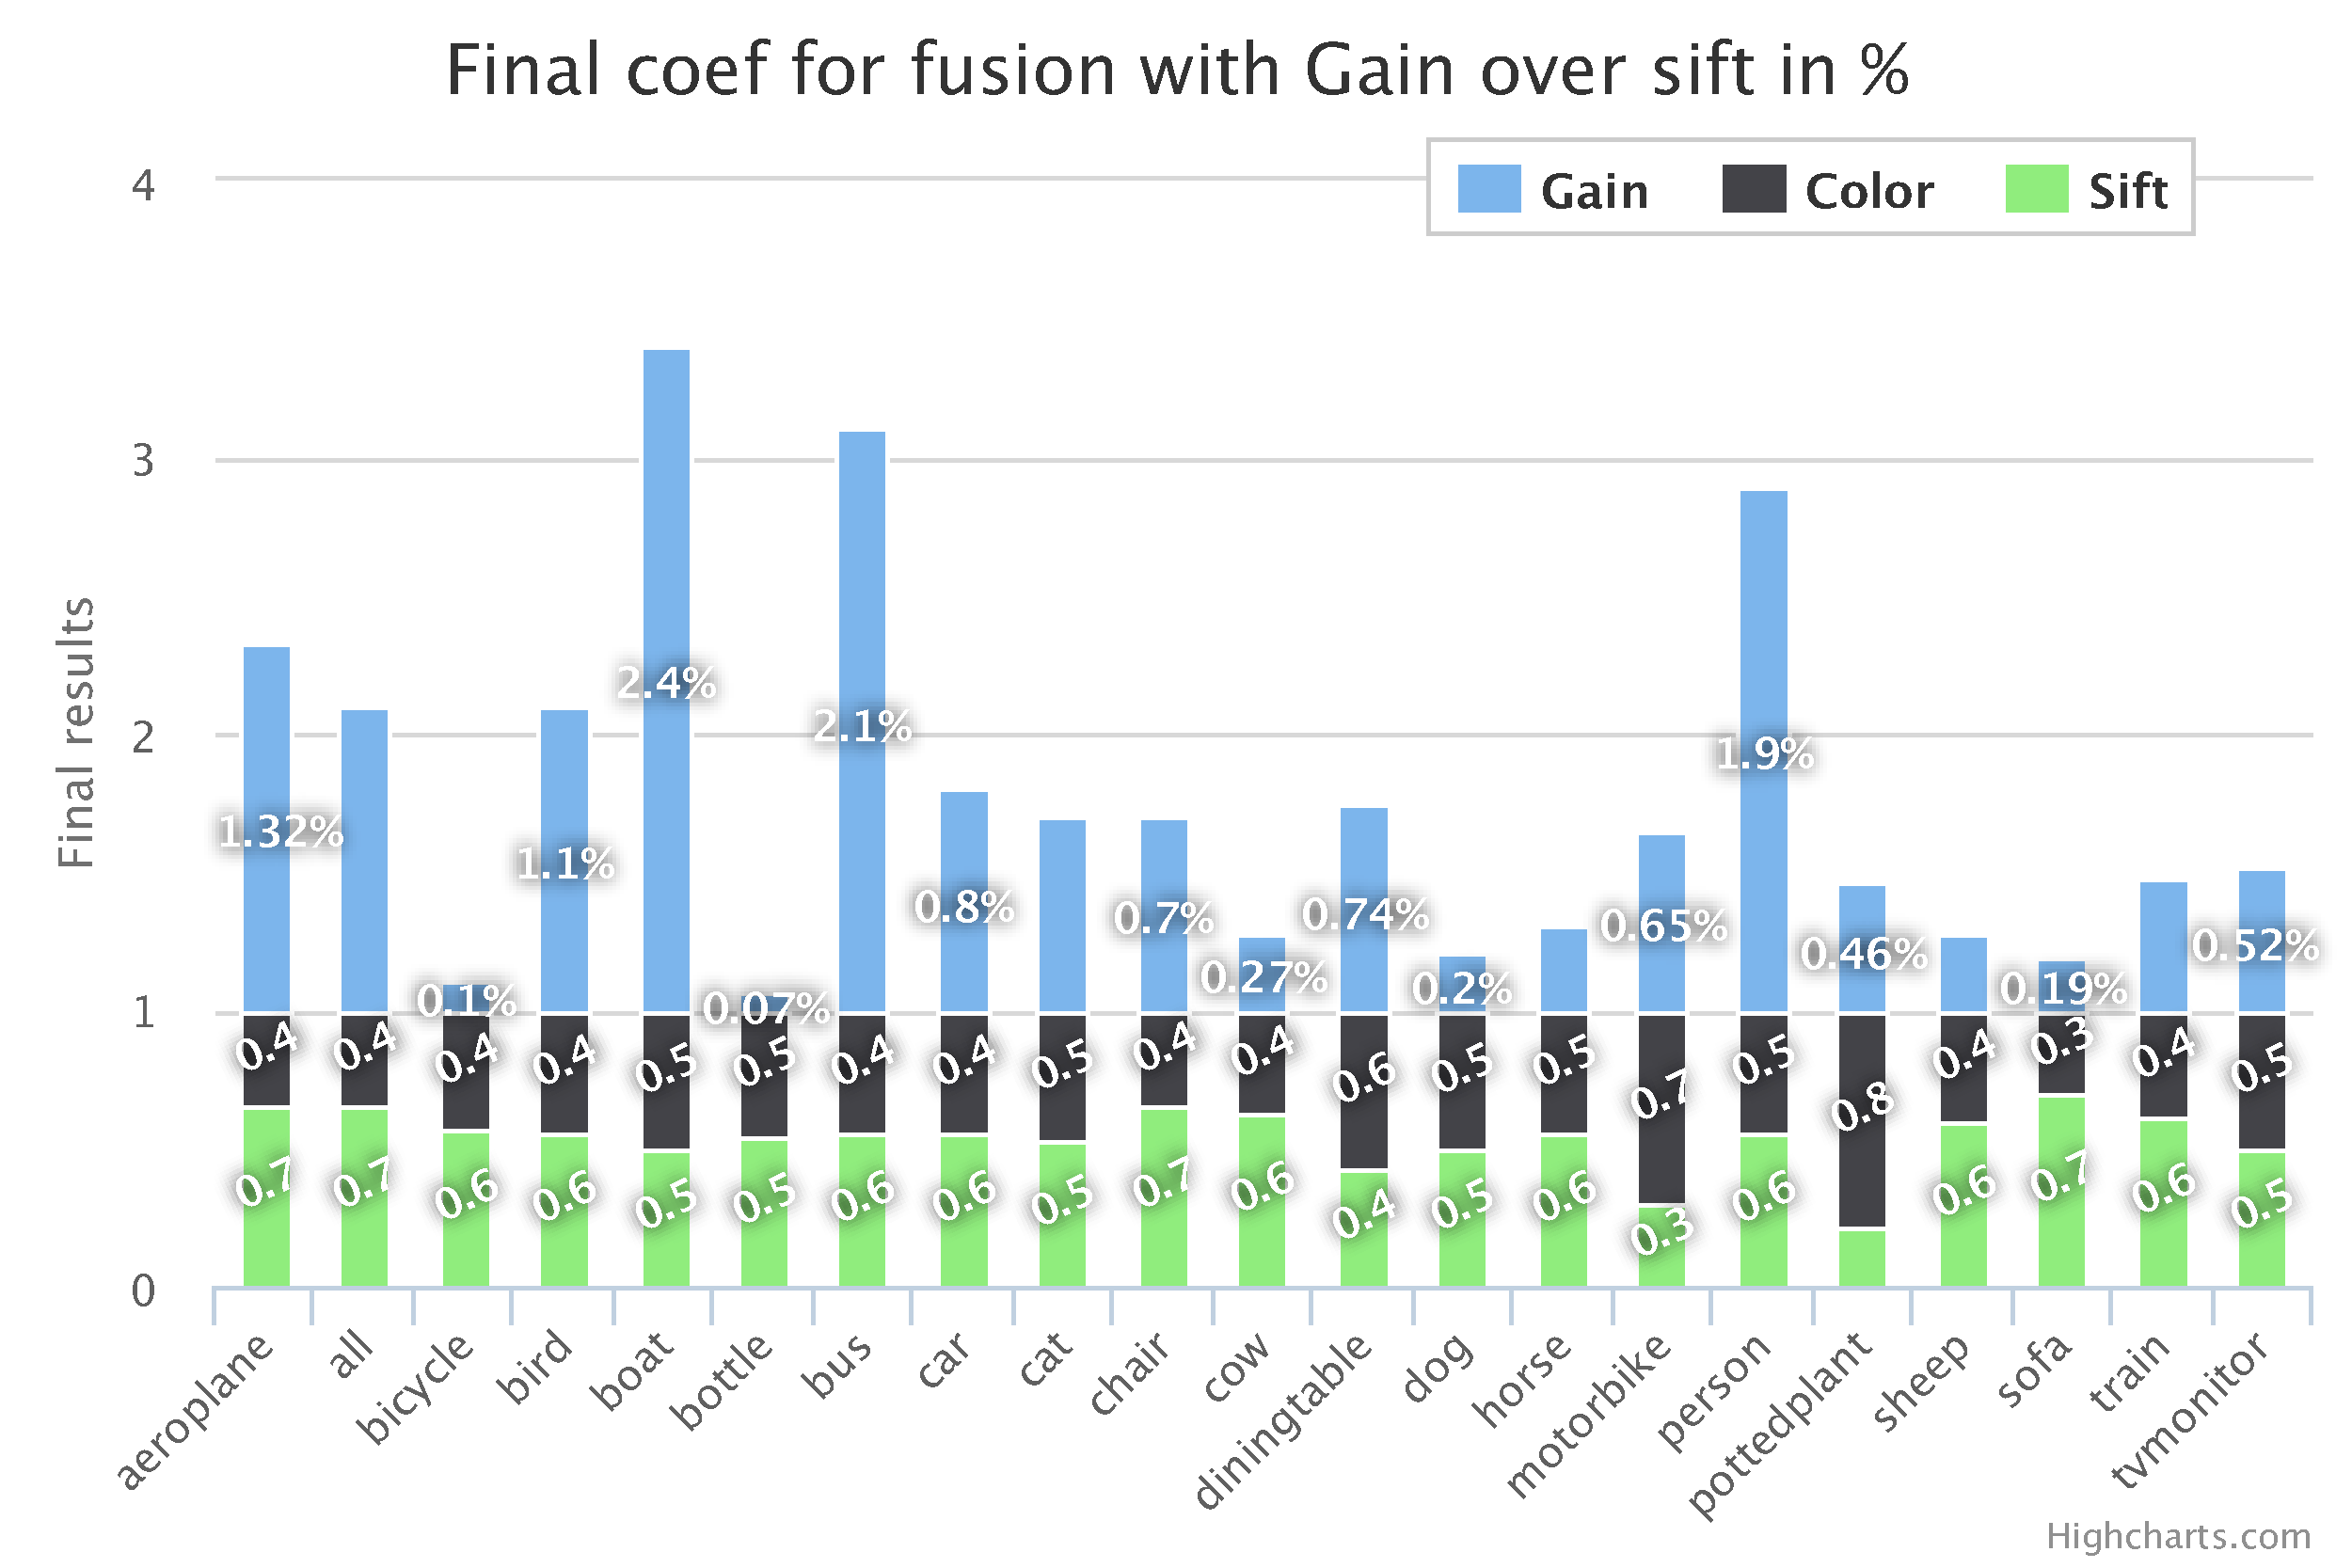
\includegraphics[scale=0.41]{fusion_coef.pdf}}
\end{center}

Le schéma ci-dessus décrit le gain effectif en pourcentage apporté par la fusion par rapport au résultats de sift. La valeur "Gain" est calculé avec la formule :

\begin{equation}
  Gain = (| map_{sift} - map_{fusion} | / (map_{sift} - map_{fusion}) / 2) * 100
\end{equation}

Les valeurs de sift et de color représentent les poids attribués lors de la fusion des fichiers \texttt{.out}.

\section{Evaluation d'une image}

voici Les figures 1  à trois présentes quelques résultats obtenue grace à l'interface web sur l'évaluation d'une image.
\begin{figure}[!ht]%
    \centering
    \subfloat[dining table and chair]{{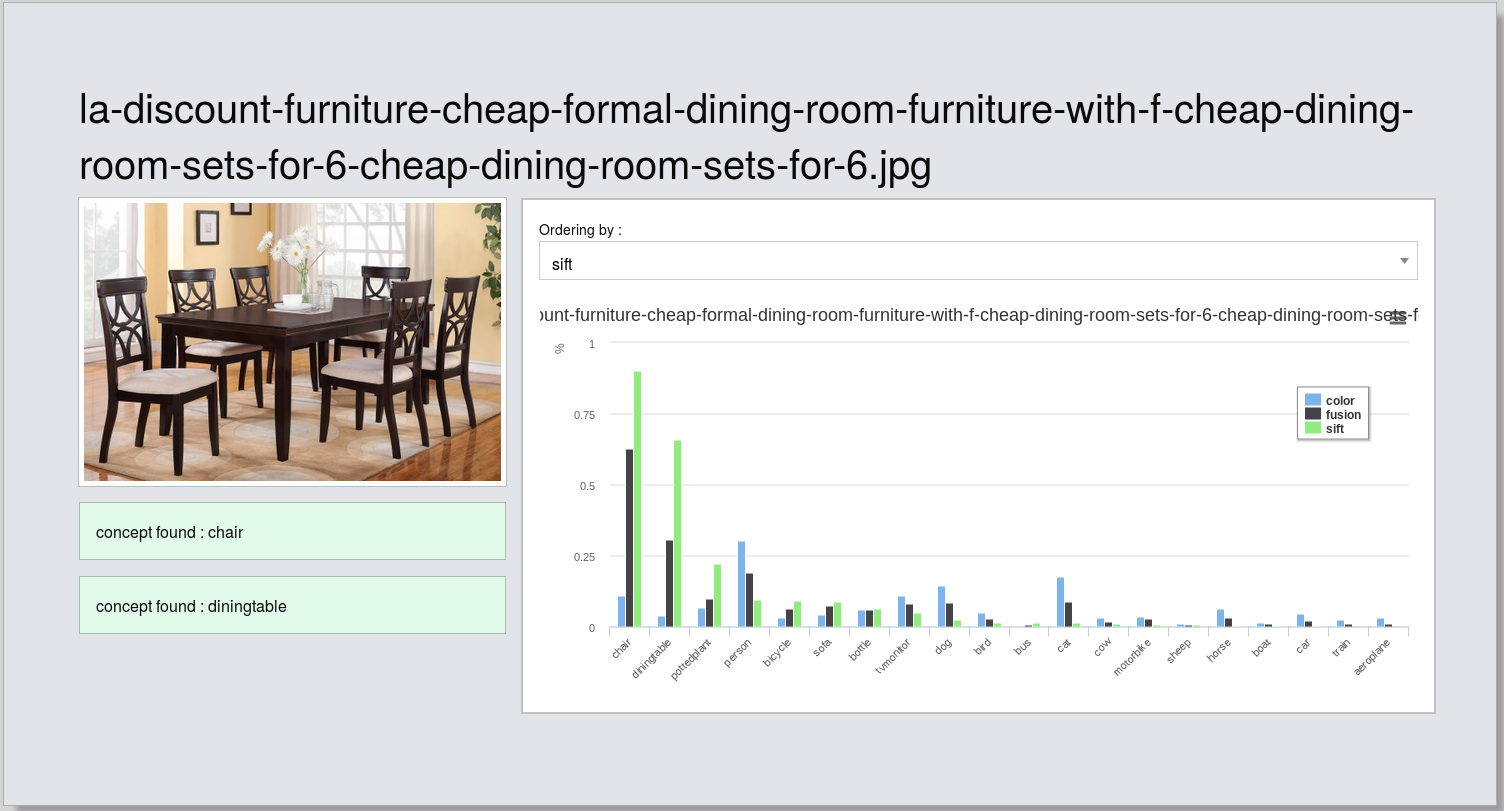
\includegraphics[scale=0.3]{process6.png} }}%
    \qquad
    \subfloat[Aeroplane]{{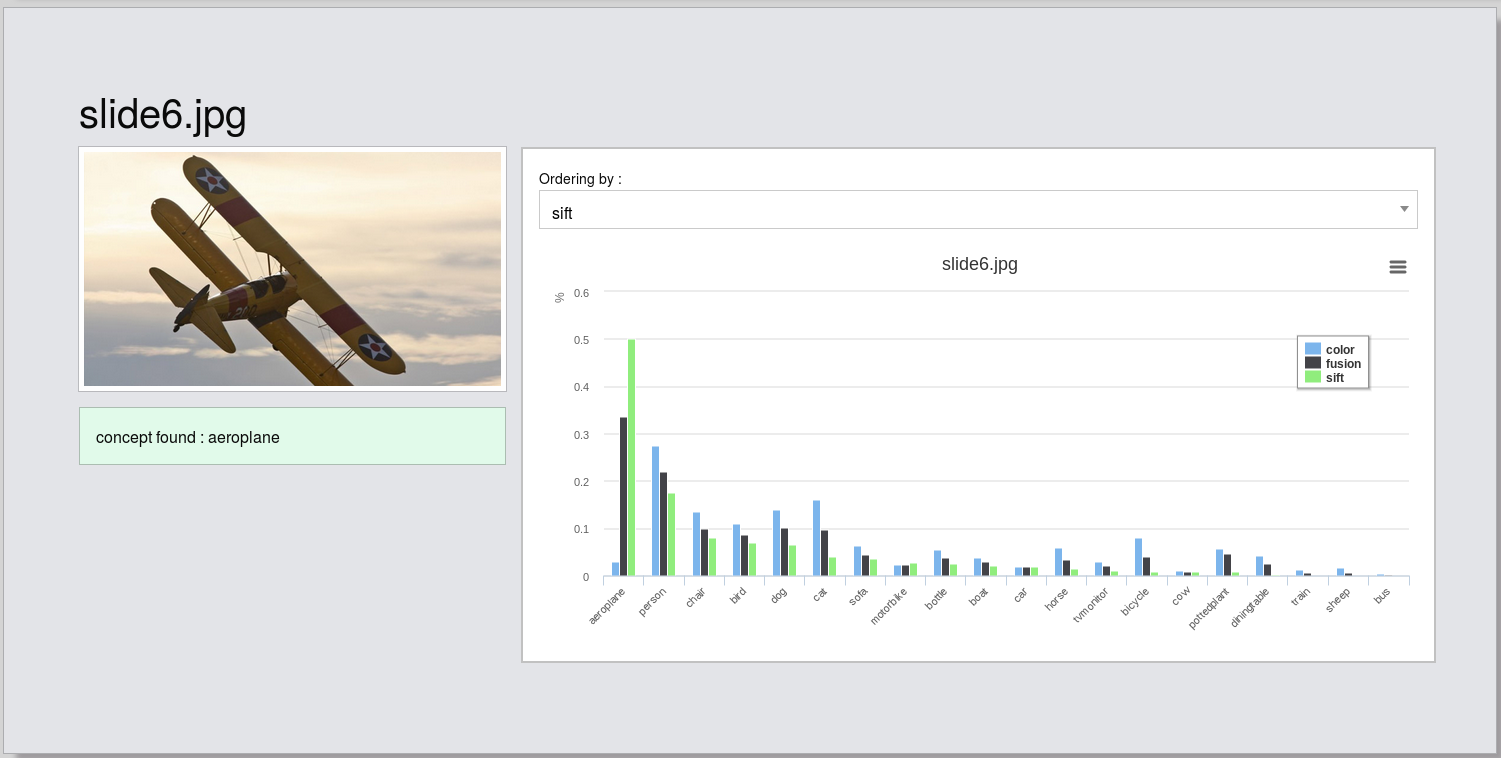
\includegraphics[scale=0.3]{process3.png} }}%
    \caption{}%
    \label{fig:example}%
\end{figure}

\begin{figure}[!ht]%
    \centering
    \subfloat[Aeroplane]{{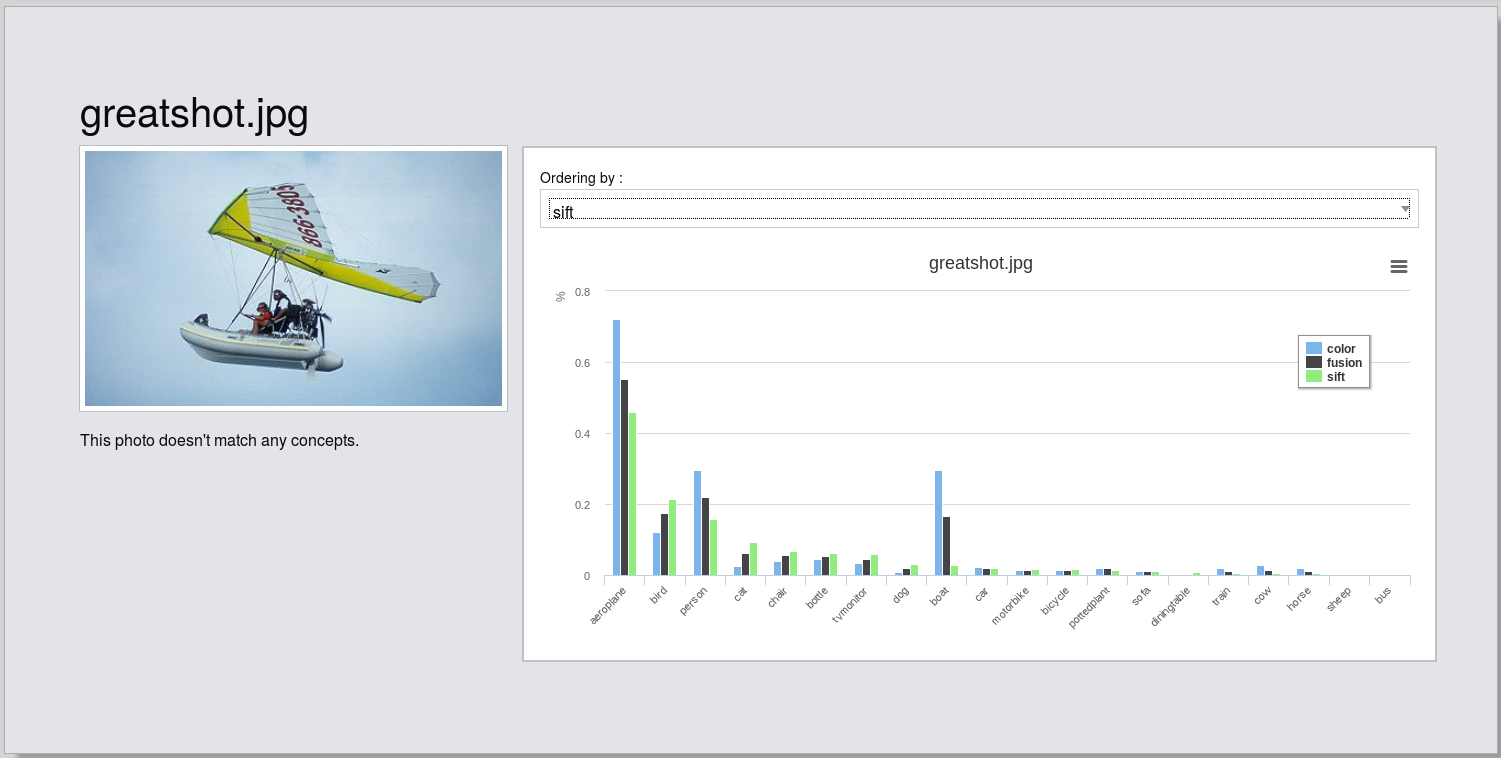
\includegraphics[scale=0.3]{process4.png} }}%
    \qquad
    \subfloat[Train]{{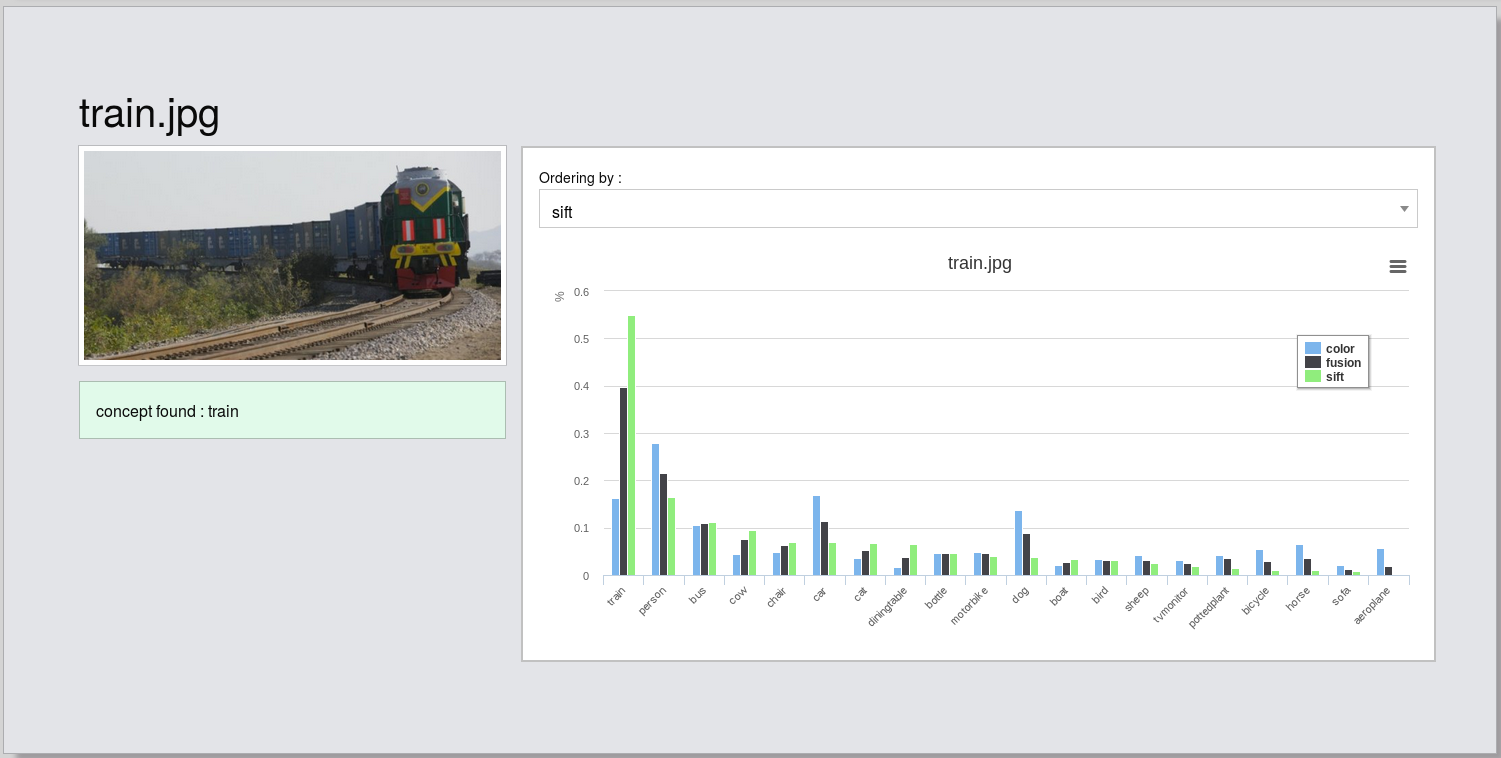
\includegraphics[scale=0.3]{process5.png} }}%
    \caption{}%
    \label{fig:example}%
\end{figure}

\begin{figure}[!ht]%
    \centering
    \subfloat[Aeroplane - une Anomalie]{{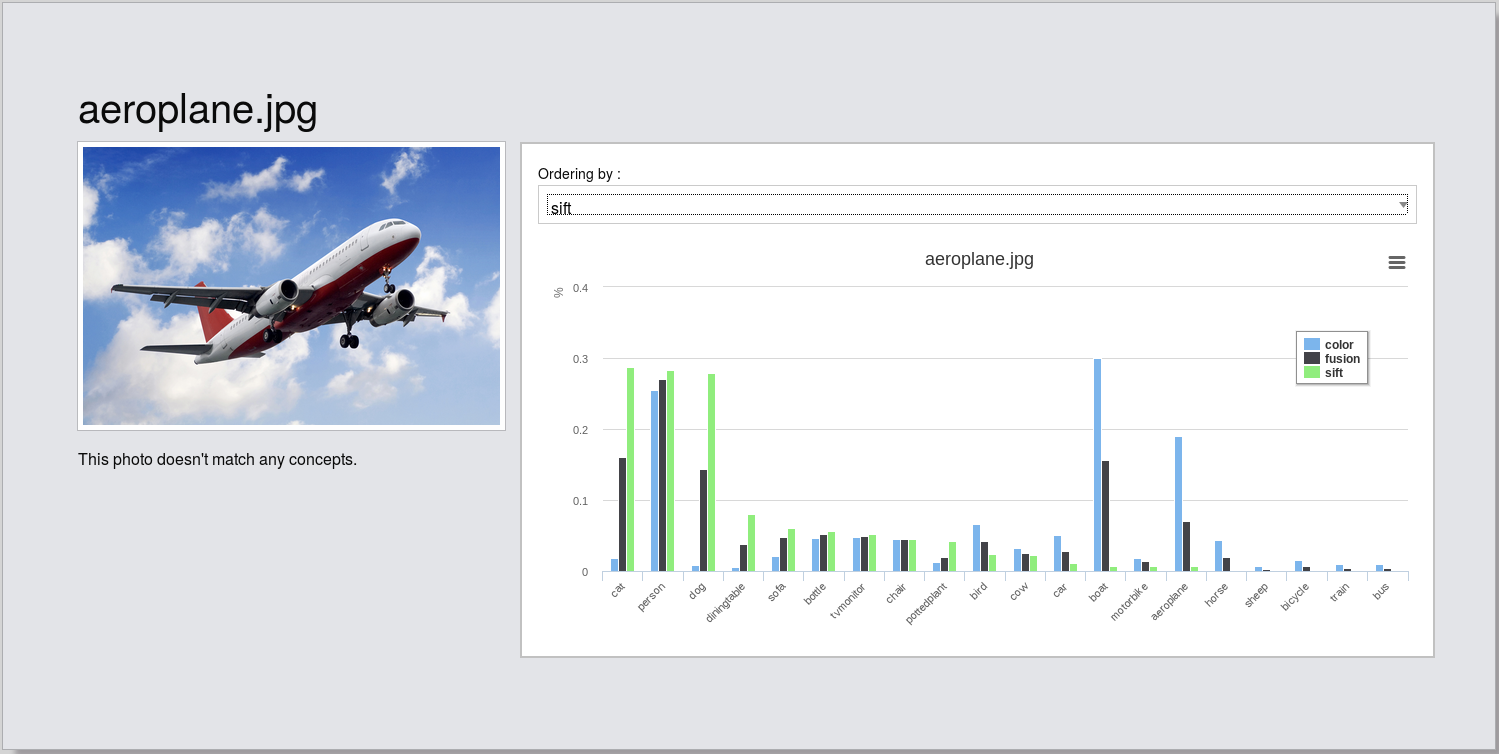
\includegraphics[scale=0.3]{process7.png} }}%
    \qquad
    \subfloat[Un centaure]{{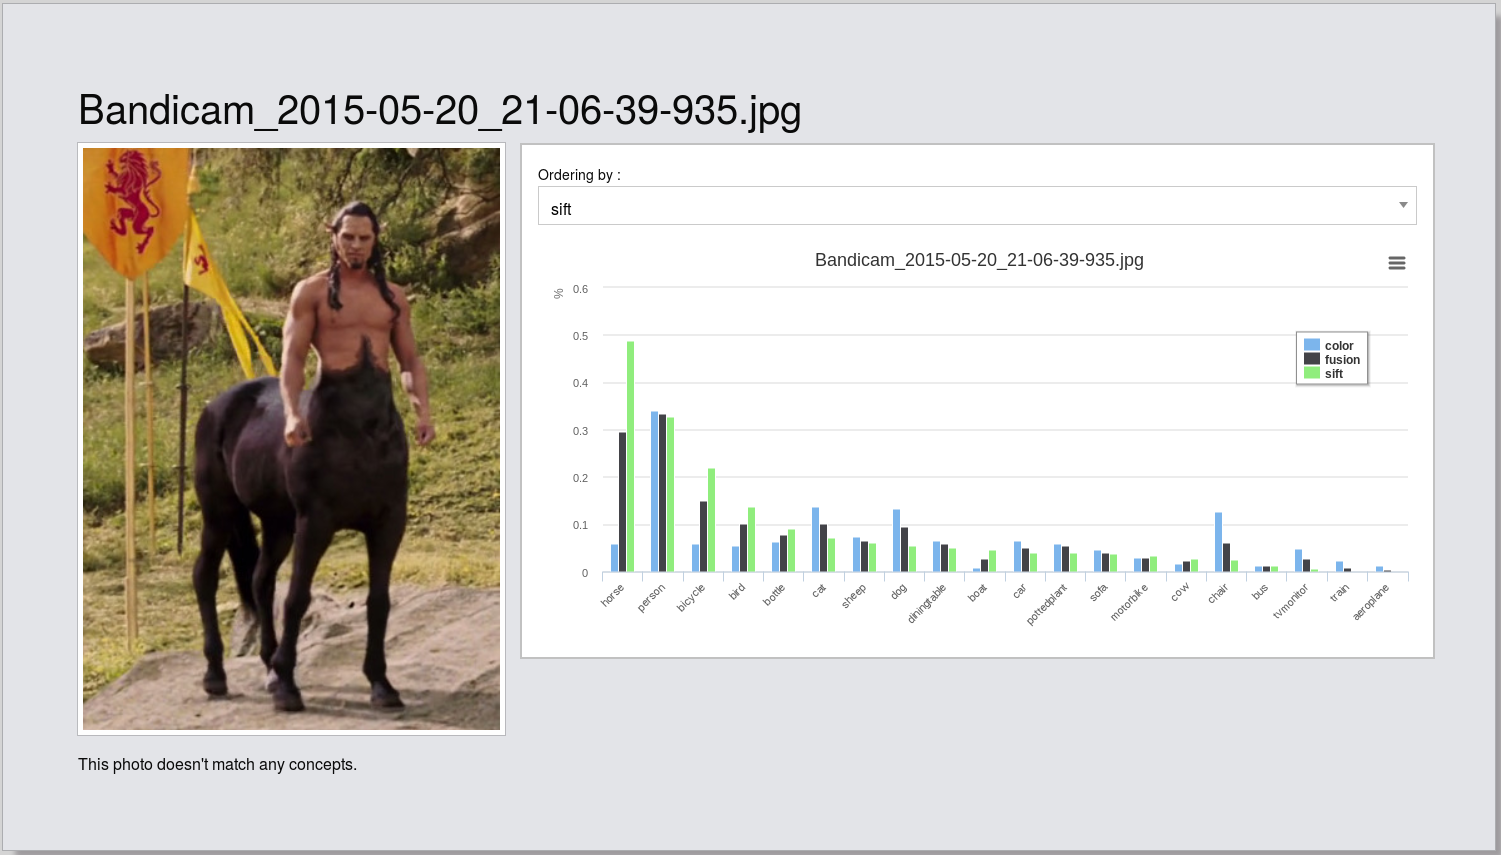
\includegraphics[scale=0.3]{process8.png} }}%
    \caption{}%
    \label{fig:example}%
\end{figure}


\end{document}
